% !TeX spellcheck = en_US
\documentclass[10pt,a4paper]{article}

% Loading packages 
\usepackage{autofe}
\usepackage{hyperref}
\hypersetup{
	colorlinks=true,
	linkcolor=blue,
	filecolor=magenta,      
	urlcolor=cyan
}
\usepackage{amsmath}
\usepackage{amssymb}
\usepackage{bbm}
\usepackage{stmaryrd}
\usepackage[main=english]{babel}
\usepackage{csquotes}
\usepackage{listings}
\usepackage{lstautogobble}
\usepackage{svg}
\usepackage{tikz}
\usepackage{multirow}
\usepackage{multicol}
\usepackage{tcolorbox}
\usepackage{mdframed}
\usepackage{proof}
\usepackage{biblatex}
\usepackage{xparse}
\usepackage{cprotect}
\usepackage{titlesec}
\usepackage{xpatch}
\usepackage{enumitem}
\usepackage{amsfonts}
\usepackage{mathtools}
\usepackage[page,header]{appendix}
\usepackage{minitoc}
\usepackage{mathtools}
\usepackage{textgreek}

\usepackage{geometry}

\usepackage{csquotes}
\usepackage[lighttt]{lmodern}
\usetikzlibrary{shapes.geometric,positioning}

% Macros caractères globales
\newcommand{\pgrph}{\P}
\newcommand{\hsep}{\vspace{.2cm}\centerline{\rule{0.8\linewidth}{.05pt}}\vspace{.4cm}}
\renewcommand{\P}{\mathbb{P}}
\newcommand{\E}{\mathbb{E}}
\newcommand{\1}{\scalebox{1.2}{$\mathbbm{1}$}}
\newcommand{\floor}[1]{\left\lfloor#1\right\rfloor}
\newcommand{\littleO}{o}
\newcommand{\bigO}{\mathcal{O}}
\newcommand{\longdash}{\:\textrm{---}\:}
\newcommand\hole{\left[\raisebox{-0.25ex}{\scalebox{1.2}{$\cdot$}}\right]}
\newcommand\bracket[1]{\!\left[#1\right]}
\newcommand{\ssi}{\quad\text{\underline{ssi}}\quad}
\newcommand\eng[1]{\textit{\foreignlanguage{english}{#1}}}
\newcommand\spacebar{\;|\;}
\def\nDownarrow{\not\mspace{1mu}\Downarrow}
\let\pprec\preccurlyeq


% Création des environnement globaux
\newtheorem{theorem}{Théorème}
\newtheorem{definition}{Definition}
\newtheorem{property}{Propriété}

\newcounter{rule}
\addto\extrasfrench{%
	\renewcommand{\figureautorefname}{\textsc{Figure}}
	\renewcommand{\sectionautorefname}{Section}
	\renewcommand{\subsectionautorefname}{Sous-section}
	\renewcommand{\appendixautorefname}{Annexe}
	\renewcommand{\theoremautorefname}{Théorème}
	\providecommand\propertyautorefname{Propriété}
	\providecommand\ruleautorefname{règle}
}

% Commandes logiques globales
\newcommand{\ifnullthenelse}[3]{
	\ifnum\value{#1}=0
	#2
	\else
	#3
	\fi
}

%%% Commande \newtag permettant de changer le label d'une equation
\makeatletter
\newcommand\newtag[2]{#1\def\@currentlabel{#1}\label{#2}}
\makeatother


% Macros caractères spécifiques au document
\newcommand\Tm{\operatorname{Tm}}
\newcommand\Set{\operatorname{Set}}
\newcommand\For{\operatorname{For}}
\newcommand\Prop{\operatorname{Prop}}
\newcommand\R{\operatorname{R}}
\newcommand\lam{\operatorname{lam}}
\newcommand\app{\operatorname{app}}
\newcommand\foralli{\operatorname{\operatorname{\forall i}}}
\newcommand\foralle{\operatorname{\operatorname{\forall e}}}
\newcommand\Pf{\operatorname{Pf}\;}
\newcommand\bCon{\textbf{Con}}
\newcommand\bSet{\textbf{Set}}
\newcommand\bProp{\textbf{Prop}}

% Agda Config
\usepackage{agda}
\usepackage{newunicodechar}
\newunicodechar{∘}{\ensuremath{\mathnormal{\circ}}}
\newunicodechar{≡}{\ensuremath{\mathnormal{\equiv}}}
\newunicodechar{◇}{\ensuremath{\mathnormal{\diamond}}}
\newunicodechar{Γ}{\textGamma}
\newunicodechar{Δ}{\textDelta}
\newunicodechar{Ξ}{\textXi}
\newunicodechar{α}{\textalpha}
\newunicodechar{β}{\textbeta}
\newunicodechar{γ}{\textgamma}
\newunicodechar{δ}{\textdelta}
\newunicodechar{ε}{\textvarepsilon}
\newunicodechar{σ}{\textsigma}
\newunicodechar{π}{\textpi}
\newunicodechar{λ}{\textlambda}
\newunicodechar{▹}{\ensuremath{\mathnormal{\triangleright}}}
\newunicodechar{⊢}{\ensuremath{\mathnormal{\vdash}}}
\newunicodechar{⇒}{\ensuremath{\mathnormal{\Rightarrow}}}
\newunicodechar{∀}{\ensuremath{\mathnormal{\forall}}}
\newunicodechar{≈}{\ensuremath{\mathnormal{\approx}}}
\newunicodechar{ₜ}{\ensuremath{{}_\text{t}}}
\newunicodechar{ₚ}{\ensuremath{{}_\text{p}}}
\newunicodechar{⁰}{\ensuremath{{}^0}}


\newcommand\agda[1]{
	\small
	\begin{code}
		\input{#1}
	\end{code}
}
% Création des environnements spécifiques au document


%%% Subparaghaphs box
\newtcbox{\subparaghaphbox}{nobeforeafter,tcbox raise base, arc=9pt, outer arc=9pt, boxsep=2pt,left=2pt,right=2pt,top=2pt,bottom=2pt,boxrule=1pt,colback=white!85!orange}
\newcommand{\subparaghaphboxedcontent}[1]{\subparaghaphbox{#1}\newline}
%\titleclass{\mathcases}{straight}[\subparagraph]
\titleformat{\subparagraph}[runin]{\normalfont\normalsize\bfseries}{}{0em}{\subparaghaphboxedcontent}
\titlespacing*{\subparagraph}{0pt}{3.25ex plus 1ex minus .2ex}{0.5em}


\addbibresource{Bilibibio.bib}


\title{Logic as a Second Order Generalized Algebraic Theory
	\\[1ex] \large Notes on my 3 month internship at Faculty of Informatics (ELTE, Budapest)}
\hypersetup{pdftitle={Completeness Proof for different kinds of logical frameworks}}
\author{Samy Avrillon, supervised by
	\\[1ex] Ambrus Kaposi (ELTE, Budapest)
	\\[1ex] and Thorsten Altenkirsch (University of Notthingham, United Kingdom)}

\begin{document}
	\doparttoc
	\maketitle
	
	\hsep
	
	\tableofcontents
	
	\newpage
	
	
	\section{Introduction}
	
		In the first place, i was supposed to do this internship in Nottingham (UK) with Thorsten Altenkirsh. But, because of administrative issues, I was not able to go there, and Thorsten Altenkirsh contacted Ambrus Kaposi in Budapest, whose university agreed to accept me. Therefore, i went to Budapest and i did the internship under the physical supervision of Ambrus Kaposi, and the remote supervision of Thorsten Altenkirsch.
		
		The original subject of the internship was \enquote{Developping a simplified account of normalization by evaluation using the theory of categories with families}. But there was a lot to do, starting with learning how to use Agda.
		
		\subsection{Introduction to the problem}
			What i do call a \enquote{logic} is a set of definitions containing formulæ and a notion of provability of those formulæ, plus a set of operators/equalities to construct or reduce these proofs. I have studied the most common logical frameworks, that is, Propositional Logic, First-Order Logic with an Infinitary operator, and Predicate Logic. For each of those logics, one can define a notion of \emph{model}. A model of a certain kind of logic is something that implements all of the logic's definitions, operators and equalities. From all of those models, one can extract the \emph{initial model}, also called \emph{syntax}. It is the smallest of all models, which means that for any model of that logic, we have a morphism from the syntax to this model.
			
			Then, our goal is for each logic to prove the completeness of a specific class of models. Completeness can be stated as such: \enquote{For any formula, if it is provable in all models of the specified class, then it has a proof in the syntax}.
			
		\subsection{Motivation}
			Ambrus is currently studying Second Order Generalized Algebraic Theories (or SOGAT) and he is trying to state a better definition than that first defined in Taichi Uemura's thesis \cite{UemuraThesis2021}. He also wants to write a paper with examples to show why they are useful, and adding some examples for different frameworks of logic can help with that.
			
		\subsection{Structure of this report}
		
			In this report, i will gradually increase the complexity of the logic i am studying. I will first study the most simple Propositional logic, which will serve as an explanation the different concepts used in the report, and then i will study Predicate Logic, first in a layout using a trick to avoid most of the difficulties, and then in a more satisfying layout but which his harder to make.
			
			For each logic, we will first give the SOGAT definition of the logic. We will then transform it into a GAT (i.e. something that can be understood by Agda). Then we will construct the syntax of the logic. Finally, we will construct the completeness proof for the studied logic.
			
			Unfortunately, the proof of the initiality of Predicate Logic's syntax as well as its completeness proof are not given in this report as i did not have the time to make them at the end of the internship.
			
	\section{Propositional Logic}
		\subsection{Propositional Logic as a SOGAT}
		
			The first and most simple logical framework we can work with is that of Propositional Logic (refered as Zero Order Logic or ZOL in the code). We also work in the most simple framework in which we only have one axiom rule for creating formulæ: the \iotAgda{} rule. Propositional Logic is usually done with a fixed set of propositional variables instead of only one that is fixed, but adding them does not make the construction more interesting, only more complicated.
			
			In order to state all the definitions, functions and more importantly, all the equalities that a model of Propositional Logic has to verify, we will write down Propositional Logic as a SOGAT. It goes as described in \autoref{fig:zol-sogat}.
			
			\begin{figure}
				\begin{tcolorbox}
					\begin{center}
					\begin{tabular}{lcl}
						\For & : & \Set \\
						--- \impliesAgda --- & : & \For \agdato \For \agdato \For\\
						\iotAgda & : & \For \\
						&&\\
						\Pf & : & \For \agdato \Prop⁺ \\
						\lam & : & (\Pf{} A \agdato⁺ \Pf{} B) \agdato \Pf{} (A \impliesAgda B)\\
						\app & : & \Pf{} (A \impliesAgda B) \agdato (\Pf{} A \agdato \Pf{} B)
					\end{tabular}
				 	\end{center}
				\end{tcolorbox}
				\caption{ZOL Sogat Presentation}
				\label{fig:zol-sogat}
			\end{figure}
			
			We can see that in this Sogat, we have two sorts (\For{} and \Pf{}), each of which have two constructors. Although SOGATs can have equations in them, every SOGAT in this report will not have any.
			
			A keen eye may have seen that there should be a problem with the \lam{} constructor. Its type is indeed not strictly positive (i.e. the type \Pf{} appears to the left of an arrow in the arguments of the constructor). That's why we use a ${}^+$ on the arrow, and we use the same ${}^+$ on the sort of \Pf{}. These arrow means that \Pf{} should be \emph{locally representable}. It basically means that we have to use \emph{proof variables} to implement this SOGAT.
		
		\subsection{From a SOGAT to GAT}
		
			
			Unfortunately, Agda cannot understand SOGATs directly (yet). So we have to convert this SOGAT into a (First Order) Generalized Algebraic Theory (or GAT). I will describe the process in this section, each line of the SOGAT giving birth to a set of sorts, constructors and equations in the GAT.
			
			The first thing we need to define any SOGAT-derived GAT is a base category with a terminal object. We will call \emph{contexts} the objects of this category and \emph{substitutions} the morphisms of the category.
			
			You can see that the equations for the category ($\circ$-associativity, identity to the right and to the left) have not been written down. This is because substitutions are defined as \Prop{} objects and not \Set objects. The difference between those two kinds of objects is that the former are said to be \emph{proof-irrelevant}. You can understand it as \enquote{there is at most one object into a type that is in \Prop}. Therefore, the equality described above are trivially true, because any substitution from $\Gamma$ to $\Delta$ is equal to any other substitution from $\Gamma$ to $\Delta$. This trick of using \Prop{} instead of \Set{} will be used through the report, and it will allow us to write down (and prove) a lot less equations.
			
			\begin{tcolorbox}
				\agda{agda/ZOL-1.tex}
			\end{tcolorbox}
		
			Once we have our base category, we can start to describe the sorts that we have in our SOGAT. Every sort from the SOGAT will be translated into a functor from our base category to \Set{} (or \Prop{}, depending on the case). Therefore, we have to define an action on objects, an action on morphisms (that we will always write contra-variant, and we will use the $\_[\_]$ notation), and some equalities that we will call \emph{functorality} or \enquote{\textit{Type} respects substitution}
			
			\begin{tcolorbox}
				\agda{agda/ZOL-3.tex}
				\agdasep
				\agda{agda/ZOL-4.tex}
			\end{tcolorbox}
		
			Now, we will translate the ${}^+$ in the type of proofs. As i said before, this translates into the fact that we have \emph{proof variables}. This means that we should be able to move from a context to another context in which we added one proof variable. We call this \emph{context extension}. For proof-variables, this context extension takes one parameter, as each proof-variables is of one specific \enquote{type} (which is the formula that they prove).
			
			With those context extensions, we also have to add a way to extend substitutions (which are the morphisms from the base category). We do that by adding a \emph{comma} operator that takes a substitution and a proof and which extends the goal of the substitution. (If we see a proof context as a list of formulæ and a proof substitution as a list of proofs, the action of comma is simply to add one proof to the list). We also need to be able to extract the proof and the base substitution from a substitution into an extended context (called \emph{weakening} operation). Therefore, we add two $\pi$ projections that extract the data from the substitution. We also need some equalities, that are saying that $(\AgdaField{$\pi_p¹$} , \AgdaField{$\pi_p²$})$ and $\AgdaField{$,_p$}$ are reciprocal, plus one equality saying that the comma operator also transposes the substitution. But as both \AgdaField{Pf} and \AgdaField{Sub} are in \Prop{}, those equations are unneeded.
			
			\begin{tcolorbox}
				\agda{agda/ZOL-5.tex}
			\end{tcolorbox}
			
			The last step is to add the constructors of our objects into the algebra. We write them directly as they were presented in the SOGAT, except for the new \AgdaField{Con} parameter that we need to add to everything. We also need to add one equation for each constructor saying that the constructors do respects substitutions. And we don't add any for \AgdaField{Pf} constructors as they are unneeded as \AgdaField{Pf} are in \AgdaPrimitive{Prop}.
		
			The only one we cannot translate directly is the $\rightarrow^+$ from the \lam{} constructor from the SOGAT. To translate this \emph{locally representable application}, we transform the parameter of the arrow into a context extension of the appropriate type. Therefore, a function $\Pf\; A \rightarrow^+ \Pf\; B$ becomes a proof $\Pf\; (\Gamma \:\AgdaField{$\triangleright_p$}\, A)\; B$ (except that we have to transform B that is a $\For\;\Gamma$ into a $\For\;(\Gamma \:\AgdaField{$\triangleright_p$}\, A)$, using the \emph{weakening} substitution $\AgdaField{$\pi_p¹$}\;\AgdaField{id}\;:\;\AgdaField{Sub}\;\Gamma\;(\Gamma \:\AgdaField{$\triangleright_p$}\, X)$ for any Γ-formula $X$)
		
			\begin{tcolorbox}
				\agda{agda/ZOL-8.tex}
				\agdasep
				\agda{agda/ZOL-9.tex}
				\agdasep
				\agda{agda/ZOL-11.tex}
			\end{tcolorbox}
			
			We now have completed our definition of a model for Propositional Logic, in the SOGAT setting. Inn the meantime, we will define (categorical) morphisms between models. They are composed of mappings for every sort of the GAT, plus equations for the categorical objects (terminal object, identity and composition), for the action of the functors on morphisms ($[]f$ and $[]p$) and finally equations to say that the constructors are also transported by the morphism. A lot of those equation are not written because \AgdaField{Pf} and \AgdaField{Sub} are in \Prop{}.
			\begin{tcolorbox}
				\agda{agda/ZOL-13.tex}
				\agdasep
				\agda{agda/ZOL-15.tex}
			\end{tcolorbox}
		
		\subsection{Finding a strict Syntax}
			
			What will be the use of these morphisms ? One thing we want to do is to find the \emph{initial} model, or \emph{syntax} for this class of models. It means that we want to find a model from which, for any model $M$, there exists one and only one morphism from this model to $M$. We can also call the syntax the \emph{minimal model}, as it is the model that contains just the objects something needs to be a model of Propositional Logic.
			
			Mathematically, this model is really easy to find. We only have to take all the sorts defined in the GAT and apply a quotient on every equation of the GAT. But this is not really interesting, as the defined model would not be \emph{strict}, i.e. all equations will not be definitional. Having only strict definitions for objects allows us to study completeness while removing a lot of transport issues that make the transport hell far bigger in the completeness proof. Transport Hell will be explained in \autoref{sec:transport-hell}.
			
			So we have three things to do :
			\begin{enumerate}
				\setlength{\itemsep}{-1ex}
				\item Create a model $I$ for Propositional Logic that we think is minimal
				\item For any other model $M$, create a morphism $m_I : I \to M$
				\item Show that any morphism $I \to M$ is equal to $m_I$
			\end{enumerate}
		
			Let's get started. This framework of Propositional logic has one property that we can make use of to make the construction of the syntax much more simpler. (Actually, we don't know if we could have made the syntax with this method if we haven't had this property. We will try to investigate it further in the future). This property is that formulæ do not depend on contexts. One can understand it as \enquote{a formula is the same regardless of the proof variables associated with it, as it doesn't use any of them}. Without this property, we would have to define mutually every sort of our theory, which would be awfully complicated.
			
			The first step is to define our sorts, no difficulty, we only make one datatype constructor for each constructor in the SOGAT or in the GAT. For contexts, the only two constructors are as the terminal object of the base category, or as a context extension of another context. That's where we use the fact that formulæ don't depend on contexts: it allows us to define \AgdaDatatype{For} and \AgdaDatatype{Con} separately, but also to define \AgdaDatatype{Pf} and \AgdaDatatype{Sub} separately (the \AgdaField{lam} constructor should refer to \AgdaFunction{\_[\_]f}, but formulæ substitution is identity when formulæ do not depend on contexts). There is also another special constructor for proofs, which is that of proof variables, and which corresponds to the \enquote{constructor} which is \AgdaField{$\pi_p^2$}
			
			\begin{tcolorbox}
				\agda{agda/ZOL-I-1.tex}
				\agdasep
				\agda{agda/ZOL-I-3.tex}
			\end{tcolorbox}
		
			The next step is to define substitutions. But we will first define a weaker property than substitution called \enquote{renamings}. The two definition are put one next to the other, and we can see that when \AgdaDatatype{Sub} are a list of complete proofs, \AgdaDatatype{Ren} are only lists of proof variables (i.e. direct proofs assumed from the contexts). This weaker form of substitution is needed to define the identity substitution, as we cannot directly define it recursively for fully-featured substitutions.
			
			The projections are simply a pattern-matching against the datatype.
			
			\begin{tcolorbox}
				\agda{agda/ZOL-I-4.tex}
				\agdasep
				\agda{agda/ZOL-I-6.tex}
				\vspace{0ex}
				\agda{agda/ZOL-I-7.tex}
			\end{tcolorbox}
		
			Because we need to refer to \AgdaField{id}, and more precisely to \AgdaField{$\pi_p^1$} \AgdaField{id} in the notion of proof substitution, we first define proof \emph{renamings} so we can define \AgdaFunction{wkSub} (which is the same as \AgdaField{$\pi_p^1$} \AgdaField{id}) and only after that, we define fully featured substitution.
			
			\begin{tcolorbox}
				\agda{agda/ZOL-I-9.tex}
				\agdasep
				\agda{agda/ZOL-I-10.tex}
			\end{tcolorbox}
		
			The last step is then to define substitution composition, which is done by applying the second part of the substitution to every element of the first part.
		
			\begin{tcolorbox}
				\agda{agda/ZOL-I-11.tex}
			\end{tcolorbox}
			
			And we now have a working model for Propositional Logic. We can implement our previously defined record, and all the equation can be directly understood by Agda (\AgdaInductiveConstructor{refl} is enough proof).
			
			I won't dive into the construction of the initial morphism and the proof that it is unique, because it is a bit ugly because of some \emph{transport hell} (see \autoref{sec:transport-hell} for an explanation of the issue).
			
			Still, i give you the construction of the Con and For mappings, as they show the basic idea of these construction. The idea is simple, we pattern-match against the datatype definition of our Sort in our syntax, and for each constructor, we call the corresponding one in the algebra.
			
			And the uniqueness proof is pretty simple again because you only need to prove that the \AgdaDatatype{Con} and \AgdaDatatype{For} mappings are unique, because the other ones are in \AgdaPrimitive{Prop}, so they are automatically unique. And to prove the unicity, you split again on the sort's datatype and for each constructor, you use the fact that a morphism preserves constructors, and you have a nice proof by recursion (except it's ugly because of transport hell).
			
			\begin{tcolorbox}
				\agda{agda/ZOL-I-13.tex}
			\end{tcolorbox}
				
		\subsection{Stating and Proving Completeness}
		
			Now that we have our syntax, we can try to state and prove completeness in our specific categorical framework.
			
			The general idea of completeness proofs is to take a class of model (here we will take Kripke Models), and to state that for any formlæ that has a proof in every Kripke model, then it has a proof in the syntax. The other direction is called \emph{soundness}, but we already have proven that when we created our initial morphism. This morphism can indeed turn proofs in the syntax into proofs in any model.
			
			This completeness proof is often done by taking some specific model of the class that is said to be \emph{universal}, and by showing that you can go between proofs in the universal model and proofs from the syntax freely. We often try to distinguish two reciprocal functions: \AgdaOperator{quote} that turns a proof from the syntax into a proof in the kripke model, and an \AgdaOperator{unquote} function that does the converse.
			
			In order to state this into our categorical layout, we will use an other mapping going from the initial model to our Kripke model that is called the \emph{Yoneda mapping}. The yoneda mapping is simply defined with the following equation:
			
			\[ y(\Gamma) = \operatorname{Hom}_\mathcal{U}(-,\Gamma) = \AgdaDatatype{Sub}_\mathcal{U} \; - \; \Gamma\]
			
			This works, because in the universal model, a context is a map from contexts of the syntax to \AgdaPrimitive{Prop} (because the category is posetal).
			
			\begin{center}
				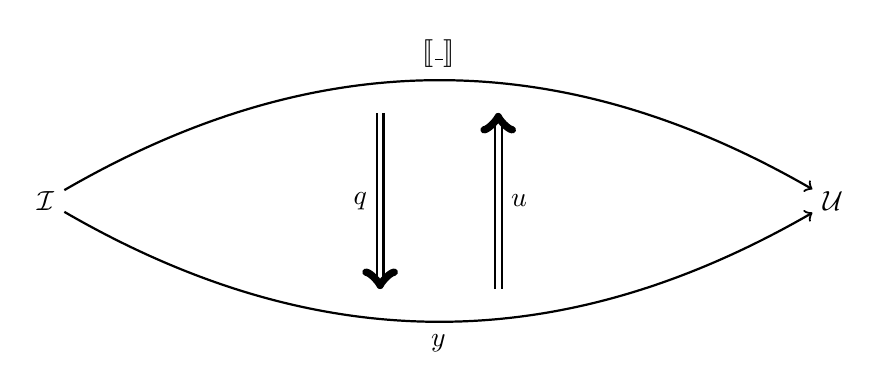
\begin{tikzpicture}[thick, scale=5]
					\node at (-1,0) (nI) {$\mathcal{I}$};
					\node at (1,0) (nU) {$\mathcal{U}$};
					
					\draw[->] (nI) to[bend left] node[midway,above,inner sep=1ex] {$\llbracket\_\rrbracket$} (nU);
					\draw[->] (nI) to[bend right] node[midway,below,inner sep=1ex] {$y$} (nU);
					
					\node at (-.15,+.25) (I0) {};
					\node at (-.15,-.25) (Y0) {};
					\draw[->,double distance=.4ex] (I0) to node[midway,left,inner sep=1ex] {$q$} (Y0);
					\node at (+.15,+.25) (I1) {};
					\node at (+.15,-.25) (Y1) {};
					\draw[->,double distance=.4ex] (Y1) to node[midway,right,inner sep=1ex] {$u$} (I1);
				\end{tikzpicture}
			\end{center}
			
			With this Yoneda Mapping, we want to construct two natural transformations $u$ and $q$ so that $u \circ q = id$. These two natural transformations are generalized version of completeness as we can prove the \enquote{real} completeness with the following construction.
			
			\begin{center}
			\begin{code}
				\>[4]\AgdaFunction{completeness}\AgdaSpace{}%
				\AgdaSymbol{:}\AgdaSpace{}%
				\AgdaSymbol{\{}\AgdaBound{Γ}\AgdaSpace{}%
				\AgdaBound{Δ}\AgdaSpace{}%
				\AgdaSymbol{:}\AgdaSpace{}%
				\AgdaDatatype{I.Con}\AgdaSymbol{\}}\AgdaSpace{}%
				\AgdaSymbol{→}\AgdaSpace{}%
				\AgdaSymbol{(\{}\AgdaBound{Ξ}\AgdaSpace{}%
				\AgdaSymbol{:}\AgdaSpace{}%
				\AgdaDatatype{I.Con}\AgdaSymbol{\}}\AgdaSpace{}%
				\AgdaSymbol{→}\AgdaSpace{}%
				\AgdaOperator{\AgdaFunction{⟦}}\AgdaSpace{}%
				\AgdaBound{Γ}\AgdaSpace{}%
				\AgdaOperator{\AgdaFunction{⟧c}}\AgdaSpace{}%
				\AgdaBound{Ξ}\AgdaSpace{}%
				\AgdaSymbol{→}\AgdaSpace{}%
				\AgdaOperator{\AgdaFunction{⟦}}\AgdaSpace{}%
				\AgdaBound{Δ}\AgdaSpace{}%
				\AgdaOperator{\AgdaFunction{⟧c}}\AgdaSpace{}%
				\AgdaBound{Ξ}\AgdaSpace{}%
				\AgdaSymbol{)}%
				\>[99]\AgdaSymbol{→}\AgdaSpace{}%
				\AgdaDatatype{I.Sub}\AgdaSpace{}%
				\AgdaBound{Γ}\AgdaSpace{}%
				\AgdaBound{Δ}\<%
				\\
				%
				\>[4]\AgdaFunction{completeness}\AgdaSpace{}%
				\AgdaSymbol{\{}\AgdaBound{Γ}\AgdaSymbol{\}}\AgdaSpace{}%
				\AgdaSymbol{\{}\AgdaBound{Δ}\AgdaSymbol{\}}\AgdaSpace{}%
				\AgdaBound{f}\AgdaSpace{}%
				\AgdaSymbol{=}\AgdaSpace{}%
				\AgdaFunction{q}\AgdaSpace{}%
				\AgdaBound{Δ}\AgdaSpace{}%
				\AgdaBound{Γ}\AgdaSpace{}%
				\AgdaSymbol{(}\AgdaBound{f}\AgdaSpace{}%
				\AgdaSymbol{\{}\AgdaBound{Γ}\AgdaSymbol{\}}\AgdaSpace{}%
				\AgdaSymbol{(}\AgdaFunction{u}\AgdaSpace{}%
				\AgdaBound{Γ}\AgdaSpace{}%
				\AgdaBound{Γ}\AgdaSpace{}%
				\AgdaFunction{I.id}\AgdaSymbol{))}\<%
			\end{code}
			\end{center}
		
		This construction means \enquote{for any list of formulæ $\Delta$ which are proven in the universal model in the context $\Gamma$ (the data of these proofs is $f$), we have a list of proofs \emph{in the syntax} of the formulæ of $\Delta$ in the context $\Gamma$}. This is exactly completeness !
		
		You can notice that we have only worked with negative fragments of logic (i.e. without disjunction), because then, Kripke models would not have been sufficient to make the completeness proof. This is another way to extend the work done during this internship.
		
	\section{First order logic (or Predicate Logic)}
	
		In this part, we will try to implement the same as we did for Propositional Logic, but this time for Predicate Logic. We again work in a simpler layout where we don't have function symbols and only have one binary relation \AgdaField{R}. And again, adding other relations and function symbols don't add a lot of new interesting content, but makes everything less readable and more complex to use.
		
		\subsection{Infinitary First Order Logic}
		
			A really naive version of first order logic can be done by implementing $\forall$ as a infinitary \enquote{and} operator. I have implemented this solution, and we can look at what it added to the code.
		
			The trick is to use an external set of terms, that is a parameter of the algebra (and therefore of all the models). This external set is called $\operatorname{TM}$.
			
			The SOGAT for this new logic is given in \autoref{fig:ifol-sogat}. We can see that we added one constructor for formulæ: $\forall$ that takes as input a function from our external $\operatorname{TM}$ to formulæ, and makes this function into a formula. We also add the introduction and elimination rule for $\forall$. We don't need to put a plus on this arrow as the set on which the recurring is external, so we don't have any strict positivity problem.
			
			\begin{figure}
				\begin{tcolorbox}
					\begin{center}
						\begin{tabular}{lcl}
							\For & : & \Set \\
							--- \impliesAgda --- & : & \For \agdato \For \agdato \For \\
							\R & : & TM \agdato TM \agdato \For \\
							\forallAgda & : & (TM \agdato \For) \agdato \For \\
							&&\\
							\Pf & : & \For \agdato \Prop⁺ \\
							\lam & : & (\Pf{} A \agdato⁺ \Pf{} B) \agdato \Pf{} (A \impliesAgda B) \\
							\app & : & \Pf{} (A \impliesAgda B) \agdato (\Pf{} A \agdato \Pf{} B) \\
							\foralli & : & (t : TM \agdato \Pf{} A t) \agdato \Pf{} (\forallAgda A)\\
							\foralle & : & \Pf{} (\forallAgda A) \agdato (t : TM) \agdato \Pf{} (A\;t)\\
						\end{tabular}
					\end{center}
				\end{tcolorbox}
				\caption{IFOL Sogat Presentation}
				\label{fig:ifol-sogat}
			\end{figure}
	
			Therefore, the GAT we deduce from this is not really more complex, we simply have to add the operators as they were described in the SOGAT together with their functorality equalities for the types that are not in \AgdaPrimitive{Prop}.
			
			\begin{tcolorbox}
				\agda{agda/IFOL-1.tex}
				\agdasep
				\agda{agda/IFOL-3.tex}
			\end{tcolorbox}
		
			The same goes to add the constructors from the syntax, this is pretty straightforward. We add a simple constructor taking a function from $\operatorname{TM}$ to \AgdaDatatype{For}, and two proofs constructors which don't break strict positivity as \AgdaInductiveConstructor{$\forall i$} takes as input a \enquote{list of proofs indexed by TM}.
			
			We also need to add cases for proof substitutions but they are really trivial cases. The same goes for the initial morphism and the proof of initiality, feel free to look at the code if you want to check it.
			
			%TODO add ref to code on internet and in appendix
			
			\begin{tcolorbox}
				\agda{agda/IFOL-I-1.tex}
				\agdasep
				\agda{agda/IFOL-I-3.tex}
			\end{tcolorbox}
			
			And Completeness proof is not harder, we just have to add the Kripke interpretation of this external forall, which is very natural, and we also need to add a case for \AgdaInductiveConstructor{$\forall$} to the definition of $u$ and $q$.
			
			We now have something that mimics first-order logic, but because the set of terms is external, the non-formulæ variables (the term variables) do not exist in our language. This logic is then not really first-order, and a more correct name might have been \enquote{Zero Order Logic with one Infinitary Operator}. Still, this construction is much more simpler than the real Predicate Logic that is presented in next section.
		
		\subsection{(Finitary) Predicate Logic as a SOGAT}
		
		\subsubsection{Making the SOGAT}
		
			The first step is again to create the SOGAT of Predicate Logic. The SOGAT is given \autoref{fig:ffol-sogat}. We can see that \emph{terms} are now part of the theory, and we see that they have to be locally representable (into $\AgdaPrimitive{Set}^+$). This is because the proof constructor \AgdaInductiveConstructor{$\forall i$} now has a strictly positive arrow, because Term are not external anymore.
			
			Except for this difference, the two SOGAT for infinitary and finitary first order logic looks very similar, and this is a great example to show that SOGATs are a good way of describing models.
		
			\begin{figure}
			\begin{tcolorbox}
				\begin{center}
					\begin{tabular}{lcl}
						\Tm & : & \Set⁺ \\
						&&\\
						\For & : & \Set \\
						--- \impliesAgda --- & : & \For \agdato \For \agdato \For \\
						\R & : & \Tm \agdato \Tm \agdato \For \\
						\forallAgda & : & (\Tm \agdato \For) \agdato \For \\
						&&\\
						\Pf & : & \For \agdato \Prop⁺ \\
						\lam & : & (\Pf{} A \agdato⁺ \Pf{} B) \agdato \Pf{} (A \impliesAgda B) \\
						\app & : & \Pf{} (A \impliesAgda B) \agdato (\Pf{} A \agdato \Pf{} B) \\
						\foralli & : & (t : \Tm \agdato⁺ \Pf{} A t) \agdato \Pf{} (\forallAgda A)\\
						\foralle & : & \Pf{} (\forallAgda A) \agdato (t : \Tm) \agdato \Pf{} (A\;t)\\
					\end{tabular}
				\end{center}
			\end{tcolorbox}
			\caption{FFOL Sogat Presentation}
			\label{fig:ffol-sogat}
			\end{figure}
			
		\subsubsection{Making a GAT out of it}
			
			So now that we want to encode a GAT from this SOGAT, we can follow the same process as we followed before. One difference is that \AgdaField{Sub} now have to be in \AgdaPrimitive{Set}, and so we have a lot more equations that were trivial before. For example, the base category now has to make explicit all the categorical equations.
			
			\begin{tcolorbox}
				
				\agda{agda/FFOL-1.tex}
				
			\end{tcolorbox}
		
			We also have to add a term extension operator like we did for formula extension. One difference is that this new kind of extension has no parameter. However, it makes it so \AgdaField{Sub} have to be in \AgdaPrimitive{Set}, and so we have to add a lot of equation concerning the two term extensions.
			
			Please ignore the \AgdaFunction{substP} for now, this notion will be explained in \autoref{sec:transport-hell}, you can just consider that this function returns its third argument unchanged and ignore the two firsts.
			
			\begin{tcolorbox}
				
				\agda{agda/FFOL-3.tex}
			\end{tcolorbox}
			\begin{tcolorbox}
				\agda{agda/FFOL-7.tex}
				\agda{agda/FFOL-8.tex}
				
			\end{tcolorbox}
			
			We also have to add a \Tm{} functor, that will have no other constructor than that of \AgdaField{$\pi_t^2$}. We don't need to change the other constructors except for \AgdaField{$\forall i$} in which the strictly positive application become a proof from a term-extended context, and for \AgdaField{$\forall e$} in which we have to \enquote{compute} what it means to apply a formula at some specific term.
			
			\begin{tcolorbox}
				\agda{agda/FFOL-2.tex}
				\agdasep
				\agda{agda/FFOL-14.tex}
			\end{tcolorbox}
			
		We now have a complete GAT for Predicate logic, and we already see that we have a lot more equations to prove.
		
		\subsection{Finding a Syntax for First Order Logic}
		
			Even though the new SOGAT don't seem a lot more complex than the one for IFOL, there is three reasons why making the Syntax will be much harder.
			
			\begin{enumerate}
				\item We cannot make Sub to be in \AgdaPrimitive{Prop} anymore, because we have term extensions, and terms are in \AgdaPrimitive{Set}, and therefore we have a lot more equations.
				\item We now have two parallel ways of extending contexts which squares the difficulty
				\item Formulæ now have to depend on contexts too (because they can contain terms)
			\end{enumerate}
		
			However, we can still do something that simplifies greatly the making of the syntax. We can split the $\bCon$ category in two. A first part will be related to term-extensions and the second part will be related to proof-extensions.
			
			The difficulty is that those two parts are not independent. Indeed, a proof-extension related context (or \emph{proof context}) will depend on formulæ, that will themselves depend on term-extension related contexts (or \emph{term contexts}).
		
			So, let's first define the term contexts, which simply describes how many terms they are in the context (therefore, it is isomorphic to Nat).
			
			\begin{tcolorbox}
				\agda{agda/FFOL-I-1.tex}
			\end{tcolorbox}
		
			Then, we can define already define terms (which can only be term variables, because \AgdaField{$\pi_t^2$} is the only constructor in our simplified version), and formulæ. Both types are indexed only by a \textbf{term} context, and we will need later to make them $\bCon \rightarrow \bSet$ rather than $\textbf{Cont} \rightarrow \bSet$. This follows the same reasoning we did when we said that Formulæ didn't have to depend on Contexts. Formulæ (and terms) never need to access proof variables, and that is the reason why we can do the separation.
			
			\begin{tcolorbox}
				\agda{agda/FFOL-I-3.tex}
				\agdasep
				\agda{agda/FFOL-I-4.tex}
			\end{tcolorbox}
		
			We now can define \textbf{term} substitutions. The algebra gives us two ways of constructing them: with \AgdaField{$,_t$} and as a morphism from the initial object, like in Propositional Logic. That's how we make our constructor. The two projections $\pi_t^1$ and $\pi_t^2$ are then simply obtained by eliminating the \AgdaInductiveConstructor{$,_t$} constructor and getting the first or second term. The equalities between $\pi_t¹$, $\pi_t²$ and $,_t$ can be proven easily in that layout.
			
			We also have to define the action of term substitutions on terms and formulæ. The definitions are really natural, as we just go down the formulæ to get to the term variables and transform them into the terms specified in the substitution.
			
			We also define the categorical constructors for the $\textbf{Cont}$ category, that are, the \AgdaFunction{id${}_t$} and \AgdaFunction{$\circ_t$} operators, and we obviously have to show their three categorical laws. Please note that these are not the equalities we will use in the final algebra, because they are only related to \AgdaDatatype{Subt} and not to the more general \AgdaField{Sub} (but we will surely use them later).
		
			We also show the functorality of \agdaSubst[t] and \agdaSubst{f}. One can notice we use some helper functions that are called \AgdaFunction{wk${}_t$} and \AgdaFunction{lf${}_t$}. Those stands for weakening and lifting. I don't show their definitions here, because they are only helper functions, but \AgdaFunction{wk${}_t$} means that from something going from a context $\Gamma$, we create something going from the context $\Gamma$ \AgdaInductiveConstructor{$\triangleright_t$} that does not uses the added variable. \AgdaFunction{lf${}_t$} means that we add one variable in the source, one variable in the goal, and that this variable is mapped to itself.
			
			I did not need renamings this time to define them because i don't have any term constructor aside from term variables.
			
			\begin{tcolorbox}
				\agda{agda/FFOL-I-5.tex}
				\agdasep
				\agda{agda/FFOL-I-7.tex}
				\agdasep
				\agda{agda/FFOL-I-9.tex}
				\agdasep
				\agda{agda/FFOL-I-10.tex}
			\end{tcolorbox}
		
			We can now start creating the other category related to proof variables. For that, we can define the base set of the category like we did with term contexts. But this time, our extension constructor has another parameter: The formula the added proof proves. Therefore, we have a dependency of \AgdaDatatype{Conp} on \AgdaDatatype{Cont}, because formulæ are defined in \AgdaDatatype{Cont}.
			
			This new $\textbf{Conp}$ category is in fact a functor from $\textbf{Cont}$ to $\bSet$. So we have to define its action on $\textbf{Cont}$'s morphisms. And we also have to proove that this action respects the functorality of $\textbf{Conp}$.
			
			We will finally create another operator on $\textbf{Conp}$: \AgdaFunction{$\triangleright$tp}. This operator does a term extension of a proof context, which doesn't add any information to the proofs, it only adds one unused variable to them (we substitute all the proofs with \AgdaFunction{wk${}_t$} \AgdaFunction{id${}_t$}). It can be understood as the action of the general \AgdaField{$\triangleright_t$} functor on $\textbf{Conp}$.
		
			\begin{tcolorbox}
				\agda{agda/FFOL-I-12.tex}
				\agdasep
				\agda{agda/FFOL-I-14.tex}
				\agdasep
				\agda{agda/FFOL-I-16.tex}
			\end{tcolorbox}
		
			We now have everything we need to define proofs, and we simply implement all the constructors from the GAT. You can notice that we have separated term and proof contexts in the definitions, but it is only for the sake of readability, because operations on proofs will often modify the proof context without changing the term context.
		
			\begin{tcolorbox}
				\agda{agda/FFOL-I-18.tex}
			\end{tcolorbox}	
		
			We also define the action of term-substitutions on proofs (because \AgdaDatatype{Pf} is a functor that is indexed by $\textbf{Cont}$). Terms substitutions does nothing to the proofs, they only affect formulæ and terms, which you cannot find inside a proof. So it is only changing the type of a proof from \Pf{}~$\Delta_t$~$\Delta_p$~$A$ to \Pf{}~$\Gamma_t$~$\Delta_p[\sigma_t]$~$A[\sigma_t]$.
		
			\begin{tcolorbox}
				\agda{agda/FFOL-I-19.tex}
			\end{tcolorbox}
		
			Again, before we can define proof substitutions, we need to define \emph{renamings} like we did for Propositional Logic. They allow us to define proof-weakening and the identity substitution. Those two functions are needed to define fully-featured substitutions. But please note that those proof substitutions are defined with a fixed term-context. So they are weaker than the final substitutions we well have to define for our algebra, that have to be able to be morphisms between contexts that differ on term-contexts and proof context at the same time. But this is not an issue and we can define all substitutions using only those restricted proof-substitutions.
			
			Again, these substitutions are a functor over the category $\textbf{Cont}$, so we have to construct the action on morphisms, which is simply applying the transformations to all the proofs contained in the substitution.
			
			\begin{tcolorbox}
				\agda{agda/FFOL-I-20.tex}
				\agdasep
				\agda{agda/FFOL-I-22.tex}
				\agdasep
				\agda{agda/FFOL-I-24.tex}
			\end{tcolorbox}
		
			With this new kind of substitution, we can substitute on proofs (that's what they're for). In other words, we have to describe the action of the \Pf{} functor on the morphisms of the category $\textbf{Conp}$.
			
			Proof substitution of proofs is simple to define, as we only get down the proof until we find a proof variable, in which case we replace it with the proof in the substitution, like we did for term-substitutions and formulæ.
			
			Again, we have defined \AgdaFunction{wk${}_p$} and \AgdaFunction{lf${}_p$}. The former will add an unused proof variable (an assumption) in a substitution, and the latter adds a formula in the goal which is proven using an assumption.
		
			\begin{tcolorbox}
				\agda{agda/FFOL-I-26.tex}
			\end{tcolorbox}
		
			This definition of proof substitutions allows us to define the categorical operators for proof substitutions. 
		
			Of course, we have to show that the categorical laws apply to them, that \agdaSubst{$\sigma_p$} respects them, as we did for the \AgdaInductiveConstructor{Subt}'s laws.
			
			The proofs of these laws contains a lot of transports which make them not very readable. This transport issue is explained in \autoref{sec:transport-hell}.
			
			\begin{tcolorbox}
				\agda{agda/FFOL-I-27.tex}
			\end{tcolorbox}
		
			The last step is to merge our two kinds of contexts and substitutions in order to match the algebra.
			
			For contexts, we simply have a record type containing both a \AgdaDatatype{Cont} and a \AgdaDatatype{Conp} that depends on it. But for substitutions, we defined \AgdaDatatype{Subp} to only describe substitutions between \AgdaDatatype{Conp}{\footnotesize s} with \emph{the same \AgdaDatatype{Cont}}. Our solution is to understand global substitutions as a sequence of two substitutions, first on terms, and then on proofs. That's why in the definition below, the \enquote{proof} part of the substitution can only be applied to proofs on $\Delta_p [t]$, i.e. proofs that have already been term-substituted by the \enquote{term} part of the substitution. The definition of the global proof substitution matching the shape given to the algebra is given after, and you can see that substitutions works exactly as described, first, the proof and everything inside is substituted using the \enquote{term} part of the substitution, and only after that the \enquote{proof} part of the substitution is applied.
		
			\begin{tcolorbox}
				
				\agda{agda/FFOL-I-28.tex}
				\agdasep
				\agda{agda/FFOL-I-30.tex}
				
				\agdasep
				
				\begin{code}
					\>[4]\AgdaOperator{\AgdaField{pf\AgdaSpace{}[\AgdaSpace{}\textsigma\AgdaSpace{}]p}}\AgdaSpace{}%
					\AgdaSymbol{=}\AgdaSpace{}%
					\AgdaSymbol{(}pf\AgdaSpace{}%
					\AgdaOperator{\AgdaFunction{[}}\AgdaSpace{}%
					\AgdaField{Sub.t}\AgdaSpace{}%
					\textsigma\AgdaSpace{}%
					\AgdaOperator{\AgdaFunction{]pₜ}}\AgdaSymbol{)}\AgdaSpace{}%
					\AgdaOperator{\AgdaFunction{[}}\AgdaSpace{}%
					\AgdaField{Sub.p}\AgdaSpace{}%
					\textsigma\AgdaSpace{}%
					\AgdaOperator{\AgdaFunction{]p}}\<%
				\end{code}
				
			\end{tcolorbox}
		
			And we can finally define our categorical operators for the merged version. They are only concatenation of the previously defined operators, so no hard logic here. Those constructions are obviously followed by the equations needed for the algebra.
			
			\begin{tcolorbox}
				
				\agda{agda/FFOL-I-32.tex}
				
				\agdasep
				\agda{agda/FFOL-I-33.tex}
				
			\end{tcolorbox}
		
			And we now have a working syntax for Predicate Logic. Unfortunately, i did not prove yet that it was really an initial model, because for the proof i need to work with a lot of transport hell, which are not really hard to solve, but takes a lot of time.
		
		\subsection{Transport Hell}
		
			\label{sec:transport-hell}
			
			In order for you to understand the code, i have to explain what are transports. I'll do this with the example of the definition of \AgdaFunction{id} in the Finitary First Order Logic syntax.
			
			To construct it, we use \AgdaFunction{idₜ} and \AgdaFunction{id${}ₚ$}, merged together with the constructor \AgdaInductiveConstructor{sub}. Here are the types of the different elements in an array.
			
			\begin{center}
			\renewcommand{\arraystretch}{1.2}
			\begin{tabular}{l|l}
				\AgdaFunction{id} & \AgdaRecord{Sub} (\AgdaInductiveConstructor{con} Γₜ Γₚ) (\AgdaInductiveConstructor{con} Γₜ Γₚ) \\\hline
				\AgdaFunction{idₜ} & \AgdaDatatype{Subt} Γₜ Γₜ \\
				\AgdaFunction{idₚ} & \AgdaDatatype{Subp} Γₚ Γₚ \\\hline
				\AgdaInductiveConstructor{sub} & (σ : \AgdaDatatype{Subt} Γₜ Δₜ) \\
				 & \AgdaSymbol{$\rightarrow$} \AgdaDatatype{Subp} Γₚ (Δₚ[σ]c) \\
				 & \AgdaSymbol{$\rightarrow$} \AgdaRecord{Sub} (\AgdaInductiveConstructor{con} Γₜ Γₚ) (\AgdaInductiveConstructor{con} Δₜ Δₚ) \\
			\end{tabular}
			\end{center}
		
			But if we try to construct \AgdaFunction{id}, then we will eventually end up with the following goal:
			
			\begin{center}
			\AgdaFunction{id} = \AgdaInductiveConstructor{sub} \AgdaFunction{idₜ} \textbf{?} \quad\textit{with}\qquad \textbf{?} : \AgdaDatatype{Subp} Γₚ (Γₚ[\AgdaFunction{idₜ}]c)
			\end{center}
			
			But then Agda will complain if we give it as a goal the expression \enquote{\AgdaFunction{idₚ}}. Indeed, it is not trivial for them that \AgdaDatatype{Subp} Γₚ (Γₚ[\AgdaFunction{idₜ}]c) is the same as \AgdaDatatype{Subp} Γₚ Γₚ. Even if we can easily prove the equality between those two elements of \AgdaPrimitive{Prop} (the proof of the equality is derived from the fact that Conp is a functor from $\textbf{Cont}$ to $\bSet$, and therefore it has to respect the identity of $\textbf{Conp}$).
			
			That's where transports comes in. The function name is \enquote{subst} but i call it \emph{transport} to avoit confusion with \AgdaDatatype{Sub}. Its definition is as follows:
			
			\begin{center}
				\AgdaFunction{subst} : \{A : \AgdaPrimitive{Set}\}(P : A → \AgdaPrimitive{Prop})\{a a' : A\} → a ≡ a' → P a → P a'
			\end{center}
		
			This is exactly the thing that will solve our problem. With the equality between the two elements of \AgdaPrimitive{Prop}, we can now convert \AgdaFunction{idₚ} to something that will correctly match the goal required by Agda.
			
			This section is called \enquote{Transport Hell} because those transports between equal sets can get really annoying. In former version of the syntax, the \AgdaDatatype{Subp} were \AgdaPrimitive{Set}s instead of \AgdaPrimitive{Prop}s. And that created a lot of equalities related to polymorphic functions (quite all \AgdaDatatype{Subp}'s related functions were then polymorphic, as they would depend on proof contexts). And to solve those equalities, you have to extract what are precisely the polymorphic functions you are working with. You can see those proofs on \href{https://github.com/MysaaJava/m1-internship/commit/2728c60633a80631ed7b61bbfae5c81a1e0e193a#diff-99bc55bebd36ad0afbae3c6448793992086091c5b6b25973f73dd779690d7dd2}{former versions of the syntax}, they are really long and not very interesting (as it is basically trying to tweak our equation so that Agda understands that two types are equal).
	
	\section{Summary}
	
	
	\section{Bibliography}
	\begingroup
	\renewcommand{\section}[2]{}%
	\printbibliography
	\endgroup
	
	\newpage
	\addappheadtotoc
	\appendix
	\addtocontents{toc}{\protect\setcounter{tocdepth}{-1}}
	\appendixpage
	
	\section{Agda Code}
	
\end{document} 
